\section{OWL Ontologi}
OWL \emph{(Web Ontology Language)} dijadikan sebagai rekomendasi formal oleh W3C pada 10 februari 2004 \citep{liyang_yu}. OWL dirancang untuk kompatibel dengan sintak XML. OWL merupakan pengembangan RDF dan RDFS yang menjadi rekomendasi W3C sebelumnya, oleh karena itu secara sintaksis OWL kompatibel dengan sintak RDF dan RDF Schema.

Ide awal dari pengembangan OWL berdasarkan fakta bahwa RDF Schema belum cukup kuat dalam mereperesentasikan semantik dari sebuah \emph{statement} sehingga diperlukan definisi lebih lanjut. Definisi inilah yang kemudian diperkenalkan dalam OWL. \citet*{antoniou} menjelaskan beberapa model semantik yang tidak dapat dituangkan dalam RDF Schema diantaranya :
\begin{enumerate}
	\item Cakupan \emph{(scope)} dari sebuah properti. Sebagai contoh misalnya properti atau predikat \textit{memakan}, RDFS tidak dapat membatasi range cakupan properti ini hanya untuk kelas tertentu, misalnya kita tidak dapat menyebutkan ``Sapi hanya memakan rumput'', sementara sapi sendiri merupakan \emph{instance} dari kelas binatang, dimana kelas ini tidak hanya berisi sapi saja, namun juga dapat berisi kucing, sementara kucing tidak memakan rumput.
	\item \emph{Disjoint} antar kelas. RDFS hanya menjelaskan mengenai hirarki kelas--sub-kelas, ia tidak dapat membedakan apakah dua atau lebih kelas yang berbeda atau tidak. Sebagai contoh, misalnya kita ingin mendefinisikan kelas mobil dan motor adalah dua kelas yang berbeda, yang artinya apabila \emph{x} adalah instance dari kelas motor, maka \emph{x} tidak mungkin menjadi instance dari kelas mobil. RDFS tidak memiliki properti untuk menjelaskan hal ini, ia hanya dapat menjelaskan bahwa kedua kelas tersebut adalah merupakan sub-kelas dari kelas induk yaitu kendaraan.
	\item Kelas kombinasi. RDFS tidak dapat mendefinisikan sebuah kelas baru yang merupakan gabungan (union) dari dua atau lebih kelas lain. RDFS juga tidak dapat mendefinisikan bentuk kombinasi lain seperti isrisan atau \emph{intersection} ataupun complement dari dua buah kelas yang berbeda. Misalnya kelas Kendaraan adalah gabungan dari kelas Mobil dan Motor.
\end{enumerate}
Sebuah dokumen OWL terdiri dari elemen header, elemen kelas, elemen properti, elemen resktiksi properti, elemen properti khusus, serta elemen kombinasi boolean. 

\subsection{Elemen \emph{header}}
Sesuai dengan standar aturan XML dimana sebuah file terdiri dari sebuah elemen \emph{root}, elemen \emph{root} dari OWL adalah rdf:RDF dimana pada elemen \emph{root} ini dideklarasikan pula beberapa \emph{namspace} yang menjadi standar seperti terlihat pada contoh berikut:
\lstinputlisting[firstline=13, lastline=16]{./parts/codeblock.xml}

Header terdapat diantara elemen \texttt{<owl:Ontology> </owl:Ontology>}. Header berisi informasi mengenai OWL yang bersagkutan seperti informasi versi, keterangan dan lain sebagainya. Berikut ini adalah contoh bentuk dari header OWL
\lstinputlisting[firstline=18, lastline=22]{./parts/codeblock.xml}

\subsection{Elemen kelas}
Bagian selanjutnya adalah elemen kelas, bagian ini berada diantara elemen \texttt{<owl:Class></owl:Class>}. Sebuah kelas dapat terdiri dari beberapa sub kelas, seperti pada RDF Schema, apabila sebuah kelas merupakan sub dari kelas tertentu, maka definisinya dijelaskan di dalam elemen kelas tersebut. Sebagai contoh misalnya definisi kelas berikut:
\lstinputlisting[firstline=24, lastline=27]{./parts/codeblock.xml}

Elemen kelas di atas mendefinisikan sebuah kelas bernama laki-laki yang memiliki hubungan disjoint dengan kelas perempuan dan merupakan sub-kelas dari Person. OWL memiliki beberapa properti kelas selain disjoin seperti equivalentClass yang digunakan untuk menjelaskan ekuivalensi sebuah kelas dengan kelas tertentu, disjointUnion untuk menjelaskan sebuah kelas dijoint dengan beberapa buah kelas yang digabungkan dan lain sebagainya.

\subsection{Elemen properti}
Elemen properti adalah elemen yang menjelaskan mengenai predikat dari sebuah statement, dimana predikat ini menjelaskan hubungan antar kelas atau antar instance sebuah kelas dengan nilai dari properti instance tersebut. Oleh karena itu elemen properti terdiri dari dua jenis yaitu object property dan datatype property.

\emph{Datatype property} menjelaskan hubungan antara \textit{instance} sebuah kelas dengan properti dari \textit{instance} tersebut, misalnya properti \textbf{umur} menjelaskan hubungan antara \textbf{person1} dengan sebuah literal value \textbf{"28"}. 
\lstinputlisting[firstline=29, lastline=31]{./parts/codeblock.xml}

\emph{Object property} menjelaskan hubungan antara sebuah kelas dengan kelas lainnya, misalnya properti diampuOleh menjelaskan hubungan antara kelas dosen dengan kelas matakuliah. 
\lstinputlisting[firstline=33, lastline=37]{./parts/codeblock.xml}

OWL juga memungkinkan kita untuk mendefinisikan inverse dari sebuah properti. Dari contoh di atas, elemen \texttt{<owl:inverseOf rdf:resource="\#mengampu" />} menjelaskan bahwa properti \textbf{diampuOleh} memiliki properti inverse yaitu mengampu, dimana nilai \texttt{rdfs:domain} dan \texttt{rdfs:range} dari properti mengampu merupakan kebalikan dari nilai \texttt{rdfs:domain} dan \texttt{rdfs:range} yang dimiliki oleh properti \textbf{diampuOleh}.

\subsection{Sub-bahasa OWL}
Kemampuan OWL dalam membentuk ekspresi pengetahuan yang sangat lengkap memunculkan kendala dalam hal kemampuan komputer untuk melakukan \emph{reasoning}. Waktu komputasi yang dibutuhkan dalam proses reasoning dapat tidak terhingga, oleh karena itu kelompok kerja bidang ontologi di W3C seperti yang disebutkan oleh \citet*{mcguinness_vanharmelen} membagi OWL ontologi menjadi tiga buah sub bahasa berdasarkan batasan ekspresi logika yang dapat dibentuk yaitu:
\begin{enumerate}
	\item OWL-Full
	\item OWL-DL
	\item OWL-Lite
\end{enumerate}
OWL-Lite merupakan sub-bagian dari OWL-DL, demikian juga dengan OWL-DL merupakan sub-bagian dari OWL-Full. Gambar \ref{fig:owl_subset} menunjukkan ilustrasi dari \emph{subset} OWL.
\begin{figure}[h]
	\centering
	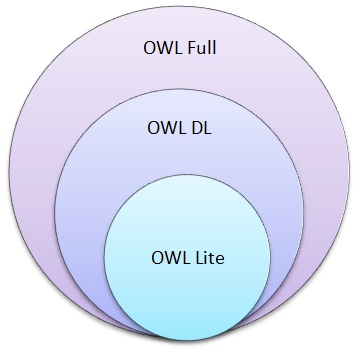
\includegraphics[width=0.5\textwidth]{owl_subset.jpg}
	\caption{Diagram venn \emph{subset} OWL 1}
	\label{fig:owl_subset}
\end{figure}